\section{aSTEP Service Design}\label{sec:service_design}
In this section, we design our service for implementation on \gls{astep}-2020. The neural network model is only part of the service as a whole.
Figure \ref{fig:service-component} shows the architectural design of the entire service. Implementing the necessary \glspl{endpoint} to allow our service to be shown in the \gls{ui} is desired, as this \gls{ui} will allow more inexperienced users access to the service. Figure \ref{fig:service-component} displays the necessary interfaces that the service must implement to be shown in the \gls{astep} \gls{ui}. This implies an interface to receive input from other services and an interface for output from the service to other services.

\begin{figure}[htbp]
    \centering
    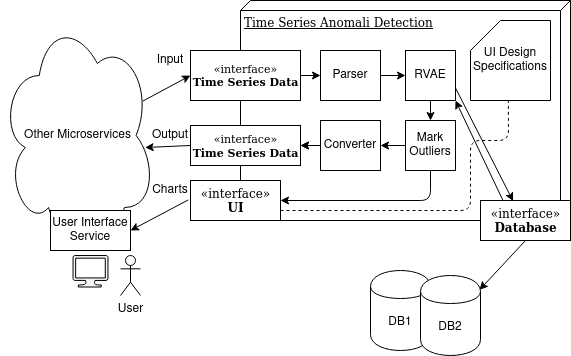
\includegraphics[width=0.85\textwidth]{Pictures/Sprint_2/ComponentArchitecture.png}
    \caption{Architecture of the service.}
    \label{fig:service-component}
\end{figure}

\subsection{Interfaces}
The interfaces to our application are:
\begin{itemize}
    \item Time Series Data
    \item UI
\end{itemize}
The interfaces are all marked in the component design figure \ref{fig:service-component} as interfaces.
The Time Series Data and \gls{ui} interfaces have been designed in collaboration with other groups and thus we have little say in how these interfaces work.

\subsection*{Time Series Data}
For the Time Series Data interface we follow the standard proposed by SW602F20, discussed in Section \ref{sc:tsinterface}. 

In the addition made to the \gls{ui}, discussed in Section \ref{sc:sap}, it was also decided that services should specify, at the \textbf{/info} \gls{endpoint}, the type of data that is expected as input, and the type of data that will be returned as output (at \textbf{/data}, \textbf{/combined}, \textbf{/render}). For the Time Series Interface, the name \textit{time-series} was chosen. The fields that are added at the \textbf{/info} \gls{endpoint} can be seen in Listing \ref{lst:info_added_fields}.

\begin{listing}[htbp]
    \begin{minted}[breaklines, linenos, escapeinside=||]{javascript}
    "input": [ {
        "name": "data-input",
        "label": "Input data",
        "type": "time-series"
    } ],
    "output": [ {
        "name": "data-output",
        "label": "Output data",
        "type": "time-series"
    } ]
    \end{minted}
    \caption{The time series interface is specified by setting it as input type.}
    \label{lst:info_added_fields}
\end{listing}

\subsubsection*{UI}
For the \gls{ui}, we must adhere to a standard, set forth by the \gls{astep}-2020 committee, that specifies some endpoints that we must expose with some specific data. In return our service will be visible within the \gls{astep} \gls{ui}.

The required endpoints are:
\begin{itemize}
    \item /info
    \item /readme
    \item /fields
    \item /render
    \item /data
    \item /combined
\end{itemize}
These endpoints must be exposed to the \gls{astep} \gls{ui} using a web server.